% Created by tikzDevice version 0.10.1 on 2016-09-01 14:32:39
% !TEX encoding = UTF-8 Unicode
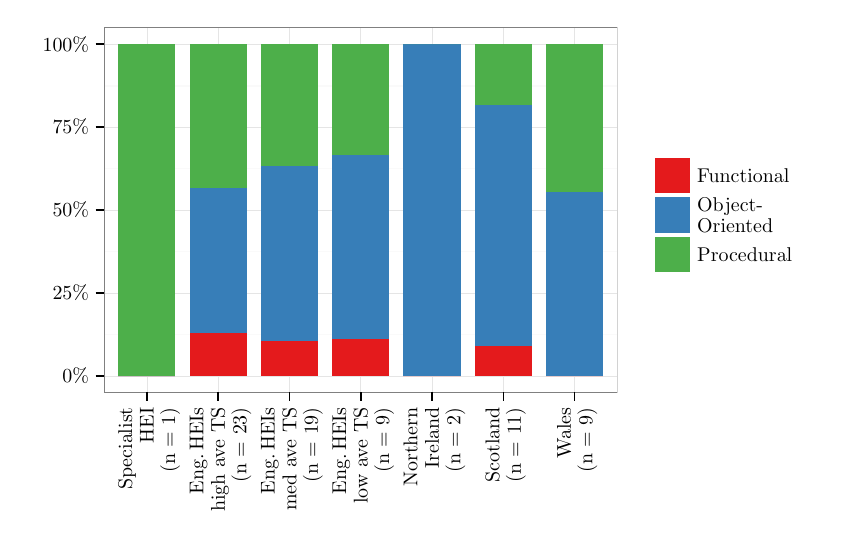
\begin{tikzpicture}[x=1pt,y=1pt]
\definecolor{fillColor}{RGB}{255,255,255}
\path[use as bounding box,fill=fillColor,fill opacity=0.00] (0,0) rectangle (289.08,180.67);
\begin{scope}
\path[clip] (  0.00,  0.00) rectangle (289.08,180.67);
\definecolor{drawColor}{RGB}{255,255,255}
\definecolor{fillColor}{RGB}{255,255,255}

\path[draw=drawColor,line width= 0.6pt,line join=round,line cap=round,fill=fillColor] (  0.00,  0.00) rectangle (289.08,180.68);
\end{scope}
\begin{scope}
\path[clip] ( 27.58, 48.88) rectangle (213.11,180.67);
\definecolor{fillColor}{RGB}{255,255,255}

\path[fill=fillColor] ( 27.58, 48.88) rectangle (213.11,180.67);
\definecolor{drawColor}{gray}{0.98}

\path[draw=drawColor,line width= 0.6pt,line join=round] ( 27.58, 69.85) --
	(213.11, 69.85);

\path[draw=drawColor,line width= 0.6pt,line join=round] ( 27.58, 99.80) --
	(213.11, 99.80);

\path[draw=drawColor,line width= 0.6pt,line join=round] ( 27.58,129.75) --
	(213.11,129.75);

\path[draw=drawColor,line width= 0.6pt,line join=round] ( 27.58,159.71) --
	(213.11,159.71);
\definecolor{drawColor}{gray}{0.90}

\path[draw=drawColor,line width= 0.2pt,line join=round] ( 27.58, 54.87) --
	(213.11, 54.87);

\path[draw=drawColor,line width= 0.2pt,line join=round] ( 27.58, 84.83) --
	(213.11, 84.83);

\path[draw=drawColor,line width= 0.2pt,line join=round] ( 27.58,114.78) --
	(213.11,114.78);

\path[draw=drawColor,line width= 0.2pt,line join=round] ( 27.58,144.73) --
	(213.11,144.73);

\path[draw=drawColor,line width= 0.2pt,line join=round] ( 27.58,174.68) --
	(213.11,174.68);

\path[draw=drawColor,line width= 0.2pt,line join=round] ( 43.04, 48.88) --
	( 43.04,180.67);

\path[draw=drawColor,line width= 0.2pt,line join=round] ( 68.81, 48.88) --
	( 68.81,180.67);

\path[draw=drawColor,line width= 0.2pt,line join=round] ( 94.58, 48.88) --
	( 94.58,180.67);

\path[draw=drawColor,line width= 0.2pt,line join=round] (120.34, 48.88) --
	(120.34,180.67);

\path[draw=drawColor,line width= 0.2pt,line join=round] (146.11, 48.88) --
	(146.11,180.67);

\path[draw=drawColor,line width= 0.2pt,line join=round] (171.88, 48.88) --
	(171.88,180.67);

\path[draw=drawColor,line width= 0.2pt,line join=round] (197.65, 48.88) --
	(197.65,180.67);
\definecolor{fillColor}{RGB}{228,26,28}

\path[fill=fillColor] ( 32.73, 54.87) rectangle ( 53.35, 54.87);
\definecolor{fillColor}{RGB}{55,126,184}

\path[fill=fillColor] ( 32.73, 54.87) rectangle ( 53.35, 54.87);
\definecolor{fillColor}{RGB}{77,175,74}

\path[fill=fillColor] ( 32.73, 54.87) rectangle ( 53.35,174.68);
\definecolor{fillColor}{RGB}{228,26,28}

\path[fill=fillColor] ( 58.50, 54.87) rectangle ( 79.11, 70.50);
\definecolor{fillColor}{RGB}{55,126,184}

\path[fill=fillColor] ( 58.50, 70.50) rectangle ( 79.11,122.59);
\definecolor{fillColor}{RGB}{77,175,74}

\path[fill=fillColor] ( 58.50,122.59) rectangle ( 79.11,174.68);
\definecolor{fillColor}{RGB}{228,26,28}

\path[fill=fillColor] ( 84.27, 54.87) rectangle (104.88, 67.48);
\definecolor{fillColor}{RGB}{55,126,184}

\path[fill=fillColor] ( 84.27, 67.48) rectangle (104.88,130.54);
\definecolor{fillColor}{RGB}{77,175,74}

\path[fill=fillColor] ( 84.27,130.54) rectangle (104.88,174.68);
\definecolor{fillColor}{RGB}{228,26,28}

\path[fill=fillColor] (110.04, 54.87) rectangle (130.65, 68.18);
\definecolor{fillColor}{RGB}{55,126,184}

\path[fill=fillColor] (110.04, 68.18) rectangle (130.65,134.75);
\definecolor{fillColor}{RGB}{77,175,74}

\path[fill=fillColor] (110.04,134.75) rectangle (130.65,174.68);
\definecolor{fillColor}{RGB}{228,26,28}

\path[fill=fillColor] (135.80, 54.87) rectangle (156.42, 54.87);
\definecolor{fillColor}{RGB}{55,126,184}

\path[fill=fillColor] (135.80, 54.87) rectangle (156.42,174.68);
\definecolor{fillColor}{RGB}{77,175,74}

\path[fill=fillColor] (135.80,174.68) rectangle (156.42,174.68);
\definecolor{fillColor}{RGB}{228,26,28}

\path[fill=fillColor] (161.57, 54.87) rectangle (182.19, 65.76);
\definecolor{fillColor}{RGB}{55,126,184}

\path[fill=fillColor] (161.57, 65.76) rectangle (182.19,152.90);
\definecolor{fillColor}{RGB}{77,175,74}

\path[fill=fillColor] (161.57,152.90) rectangle (182.19,174.68);
\definecolor{fillColor}{RGB}{228,26,28}

\path[fill=fillColor] (187.34, 54.87) rectangle (207.95, 54.87);
\definecolor{fillColor}{RGB}{55,126,184}

\path[fill=fillColor] (187.34, 54.87) rectangle (207.95,121.43);
\definecolor{fillColor}{RGB}{77,175,74}

\path[fill=fillColor] (187.34,121.43) rectangle (207.95,174.68);
\definecolor{drawColor}{gray}{0.50}

\path[draw=drawColor,line width= 0.6pt,line join=round,line cap=round] ( 27.58, 48.88) rectangle (213.11,180.67);
\end{scope}
\begin{scope}
\path[clip] (  0.00,  0.00) rectangle (289.08,180.67);
\definecolor{drawColor}{RGB}{0,0,0}

\node[text=drawColor,anchor=base east,inner sep=0pt, outer sep=0pt, scale=  0.72] at ( 22.18, 52.39) {0\%};

\node[text=drawColor,anchor=base east,inner sep=0pt, outer sep=0pt, scale=  0.72] at ( 22.18, 82.35) {25\%};

\node[text=drawColor,anchor=base east,inner sep=0pt, outer sep=0pt, scale=  0.72] at ( 22.18,112.30) {50\%};

\node[text=drawColor,anchor=base east,inner sep=0pt, outer sep=0pt, scale=  0.72] at ( 22.18,142.25) {75\%};

\node[text=drawColor,anchor=base east,inner sep=0pt, outer sep=0pt, scale=  0.72] at ( 22.18,172.20) {100\%};
\end{scope}
\begin{scope}
\path[clip] (  0.00,  0.00) rectangle (289.08,180.67);
\definecolor{drawColor}{RGB}{0,0,0}

\path[draw=drawColor,line width= 0.6pt,line join=round] ( 24.58, 54.87) --
	( 27.58, 54.87);

\path[draw=drawColor,line width= 0.6pt,line join=round] ( 24.58, 84.83) --
	( 27.58, 84.83);

\path[draw=drawColor,line width= 0.6pt,line join=round] ( 24.58,114.78) --
	( 27.58,114.78);

\path[draw=drawColor,line width= 0.6pt,line join=round] ( 24.58,144.73) --
	( 27.58,144.73);

\path[draw=drawColor,line width= 0.6pt,line join=round] ( 24.58,174.68) --
	( 27.58,174.68);
\end{scope}
\begin{scope}
\path[clip] (  0.00,  0.00) rectangle (289.08,180.67);
\definecolor{drawColor}{RGB}{0,0,0}

\path[draw=drawColor,line width= 0.6pt,line join=round] ( 43.04, 45.88) --
	( 43.04, 48.88);

\path[draw=drawColor,line width= 0.6pt,line join=round] ( 68.81, 45.88) --
	( 68.81, 48.88);

\path[draw=drawColor,line width= 0.6pt,line join=round] ( 94.58, 45.88) --
	( 94.58, 48.88);

\path[draw=drawColor,line width= 0.6pt,line join=round] (120.34, 45.88) --
	(120.34, 48.88);

\path[draw=drawColor,line width= 0.6pt,line join=round] (146.11, 45.88) --
	(146.11, 48.88);

\path[draw=drawColor,line width= 0.6pt,line join=round] (171.88, 45.88) --
	(171.88, 48.88);

\path[draw=drawColor,line width= 0.6pt,line join=round] (197.65, 45.88) --
	(197.65, 48.88);
\end{scope}
\begin{scope}
\path[clip] (  0.00,  0.00) rectangle (289.08,180.67);
\definecolor{drawColor}{RGB}{0,0,0}

\node[text=drawColor,rotate= 90.00,anchor=base east,inner sep=0pt, outer sep=0pt, scale=  0.72] at ( 37.74, 43.48) {Specialist};

\node[text=drawColor,rotate= 90.00,anchor=base east,inner sep=0pt, outer sep=0pt, scale=  0.72] at ( 45.52, 43.48) {HEI};

\node[text=drawColor,rotate= 90.00,anchor=base east,inner sep=0pt, outer sep=0pt, scale=  0.72] at ( 53.29, 43.48) {(n = 1)};

\node[text=drawColor,rotate= 90.00,anchor=base east,inner sep=0pt, outer sep=0pt, scale=  0.72] at ( 63.51, 43.48) {Eng.\,HEIs};

\node[text=drawColor,rotate= 90.00,anchor=base east,inner sep=0pt, outer sep=0pt, scale=  0.72] at ( 71.29, 43.48) {high ave TS};

\node[text=drawColor,rotate= 90.00,anchor=base east,inner sep=0pt, outer sep=0pt, scale=  0.72] at ( 79.06, 43.48) {(n = 23)};

\node[text=drawColor,rotate= 90.00,anchor=base east,inner sep=0pt, outer sep=0pt, scale=  0.72] at ( 89.28, 43.48) {Eng.\,HEIs};

\node[text=drawColor,rotate= 90.00,anchor=base east,inner sep=0pt, outer sep=0pt, scale=  0.72] at ( 97.05, 43.48) {med ave TS};

\node[text=drawColor,rotate= 90.00,anchor=base east,inner sep=0pt, outer sep=0pt, scale=  0.72] at (104.83, 43.48) {(n = 19)};

\node[text=drawColor,rotate= 90.00,anchor=base east,inner sep=0pt, outer sep=0pt, scale=  0.72] at (115.05, 43.48) {Eng.\,HEIs};

\node[text=drawColor,rotate= 90.00,anchor=base east,inner sep=0pt, outer sep=0pt, scale=  0.72] at (122.82, 43.48) {low ave TS};

\node[text=drawColor,rotate= 90.00,anchor=base east,inner sep=0pt, outer sep=0pt, scale=  0.72] at (130.60, 43.48) {(n = 9)};

\node[text=drawColor,rotate= 90.00,anchor=base east,inner sep=0pt, outer sep=0pt, scale=  0.72] at (140.81, 43.48) {Northern};

\node[text=drawColor,rotate= 90.00,anchor=base east,inner sep=0pt, outer sep=0pt, scale=  0.72] at (148.59, 43.48) {Ireland};

\node[text=drawColor,rotate= 90.00,anchor=base east,inner sep=0pt, outer sep=0pt, scale=  0.72] at (156.37, 43.48) {(n = 2)};

\node[text=drawColor,rotate= 90.00,anchor=base east,inner sep=0pt, outer sep=0pt, scale=  0.72] at (170.47, 43.48) {Scotland};

\node[text=drawColor,rotate= 90.00,anchor=base east,inner sep=0pt, outer sep=0pt, scale=  0.72] at (178.25, 43.48) {(n = 11)};

\node[text=drawColor,rotate= 90.00,anchor=base east,inner sep=0pt, outer sep=0pt, scale=  0.72] at (196.24, 43.48) {Wales};

\node[text=drawColor,rotate= 90.00,anchor=base east,inner sep=0pt, outer sep=0pt, scale=  0.72] at (204.01, 43.48) {(n = 9)};
\end{scope}
\begin{scope}
\path[clip] (  0.00,  0.00) rectangle (289.08,180.67);
\definecolor{fillColor}{RGB}{255,255,255}

\path[fill=fillColor] (221.64, 87.36) rectangle (280.54,142.19);
\end{scope}
\begin{scope}
\path[clip] (  0.00,  0.00) rectangle (289.08,180.67);
\definecolor{fillColor}{RGB}{228,26,28}

\path[fill=fillColor] (226.62,120.80) rectangle (239.43,133.60);
\end{scope}
\begin{scope}
\path[clip] (  0.00,  0.00) rectangle (289.08,180.67);
\definecolor{fillColor}{RGB}{55,126,184}

\path[fill=fillColor] (226.62,106.57) rectangle (239.43,119.37);
\end{scope}
\begin{scope}
\path[clip] (  0.00,  0.00) rectangle (289.08,180.67);
\definecolor{fillColor}{RGB}{77,175,74}

\path[fill=fillColor] (226.62, 92.34) rectangle (239.43,105.15);
\end{scope}
\begin{scope}
\path[clip] (  0.00,  0.00) rectangle (289.08,180.67);
\definecolor{drawColor}{RGB}{0,0,0}

\node[text=drawColor,anchor=base west,inner sep=0pt, outer sep=0pt, scale=  0.72] at (241.94,124.72) {Functional};
\end{scope}
\begin{scope}
\path[clip] (  0.00,  0.00) rectangle (289.08,180.67);
\definecolor{drawColor}{RGB}{0,0,0}

\node[text=drawColor,anchor=base west,inner sep=0pt, outer sep=0pt, scale=  0.72] at (241.94,114.38) {Object-};

\node[text=drawColor,anchor=base west,inner sep=0pt, outer sep=0pt, scale=  0.72] at (241.94,106.60) {Oriented};
\end{scope}
\begin{scope}
\path[clip] (  0.00,  0.00) rectangle (289.08,180.67);
\definecolor{drawColor}{RGB}{0,0,0}

\node[text=drawColor,anchor=base west,inner sep=0pt, outer sep=0pt, scale=  0.72] at (241.94, 96.27) {Procedural};
\end{scope}
\end{tikzpicture}
